\chapter{Experiments}\label{sec:experiments}

The experiments chapter walks through the goals, trials, and conclusions from each experiment, following a systematic evaluation of relay strategies across diverse configurations.

\section{Channel Model Validation}\label{sec:channel-model-validation}

\textbf{Goal:} Validate the simulation framework against closed-form theoretical BER expressions to ensure baseline accuracy before evaluating AI relays.

\textbf{Trials:} - \textbf{Topology:} SISO, MIMO 2x2 - \textbf{Modulation scheme:} BPSK - \textbf{Channel:} AWGN, Rayleigh, Rician (K=3) - \textbf{Equalizers (in MIMO only):} None (SISO), ZF, MMSE, SIC - \textbf{Demod:} Hard decision only

\textbf{Conclusion: (Equation~\ref{eq:psk16-decision})} Monte Carlo simulations match theoretical predictions within 95\% confidence intervals across all channel models and topologies. AWGN follows the expected exponential decay (Equation~\ref{eq:awgn-ber}), Rayleigh validates the \(1/(4\bar{\gamma})\) high-SNR slope (Equation~\ref{eq:rayleigh-ber-approx}), Rician falls between the two, and MIMO equalization correctly exhibits the expected ZF \textless{} MMSE \textless{} SIC performance hierarchy (Equation~\ref{eq:zf-snr}).

\subsection{Results Figures}\label{sec:results-figures}











\begin{figure}[H]
\centering
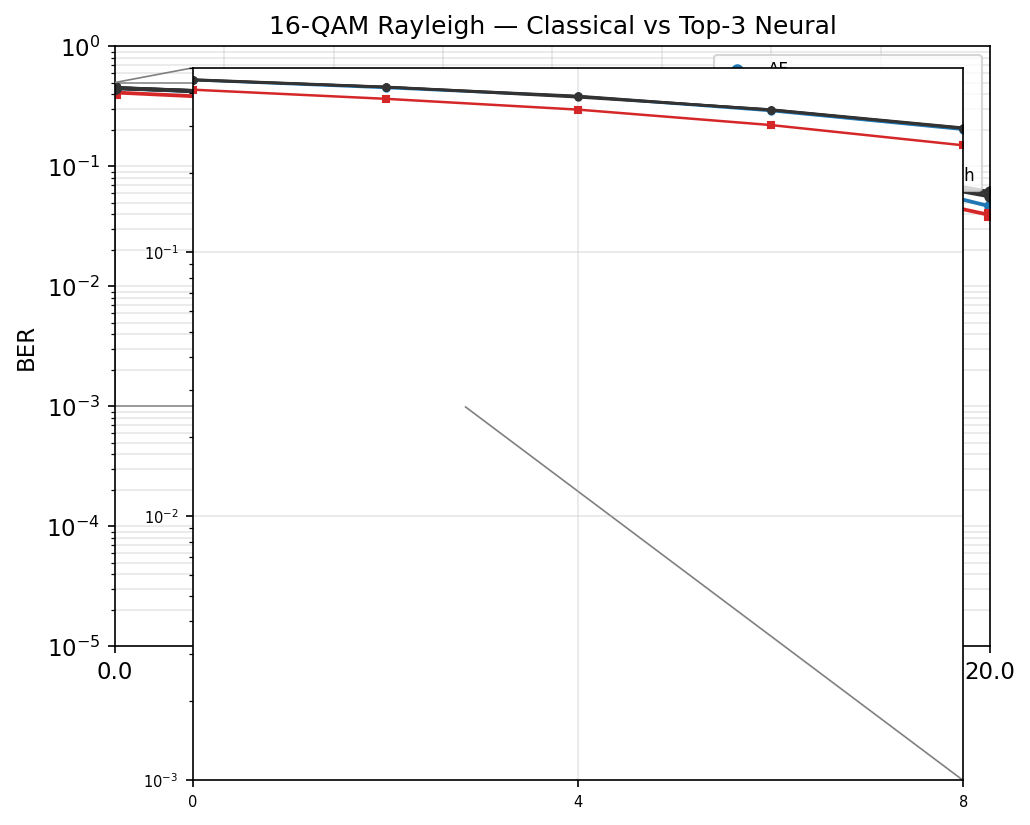
\includegraphics[width=0.92\linewidth]{results/csi/top3_qam16_rayleigh_split_1.png}
\caption{16-QAM Rayleigh --- classical relays (AF, DF) vs.~top-3 neural relay variants. Zoom inset: 0--8~dB.}
\label{fig:fig40_p1}
\end{figure}

\begin{figure}[H]
\centering
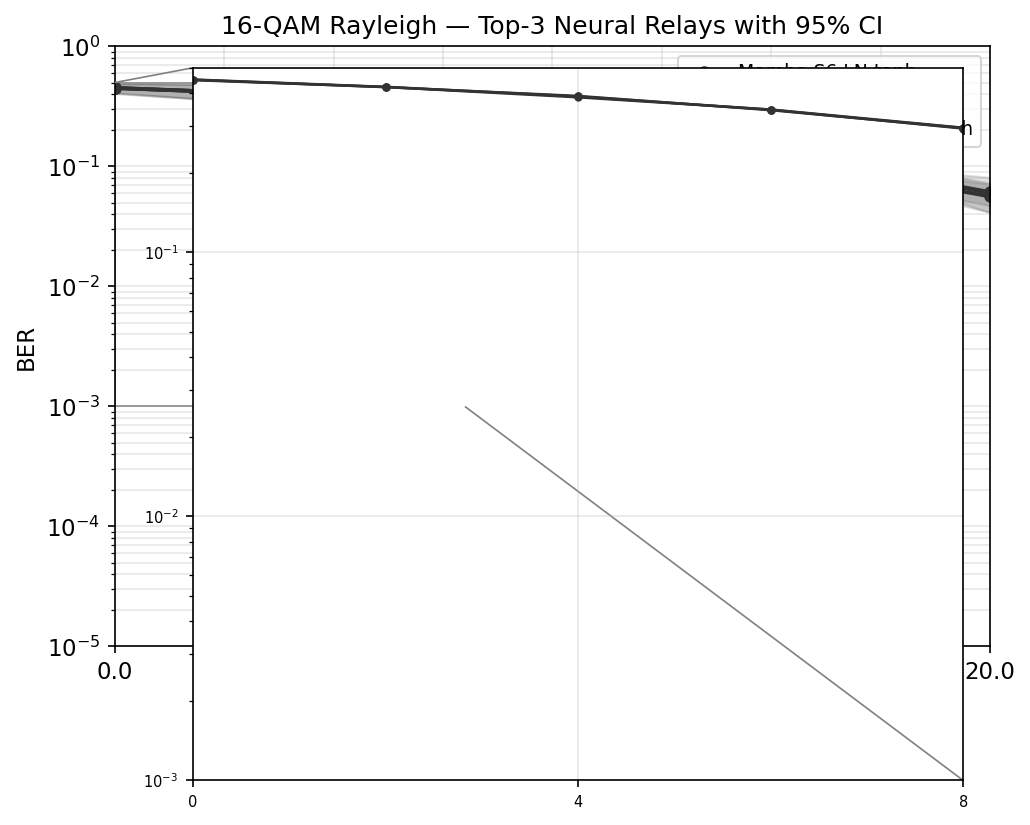
\includegraphics[width=0.92\linewidth]{results/csi/top3_qam16_rayleigh_split_2.png}
\caption{16-QAM Rayleigh --- top-3 neural relay variants with 95\% confidence intervals. Zoom inset: 0--8~dB.}
\label{fig:fig40_p2}
\end{figure}

\begin{figure}[H]
\centering
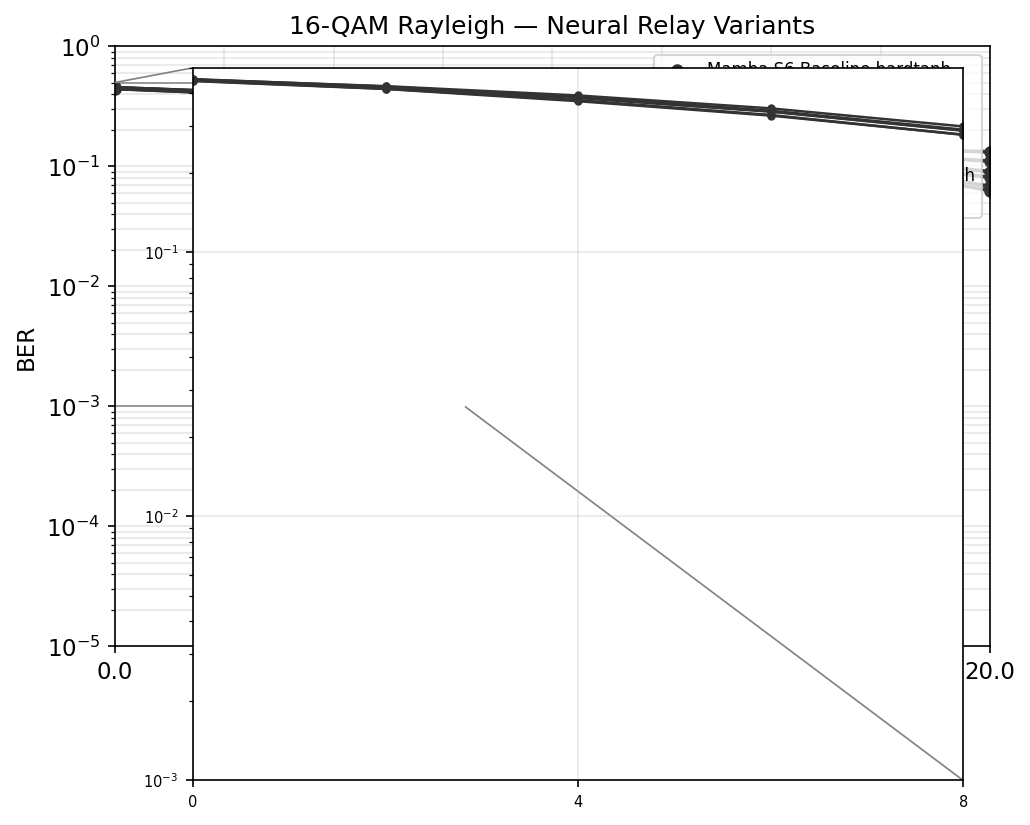
\includegraphics[width=0.92\linewidth]{results/csi/top3_qam16_rayleigh_split_3.png}
\caption{16-QAM Rayleigh --- additional neural relay variants for comparison.}
\label{fig:fig40_p3}
\end{figure}

\begin{figure}[H]
\centering
\centering
\pandocbounded{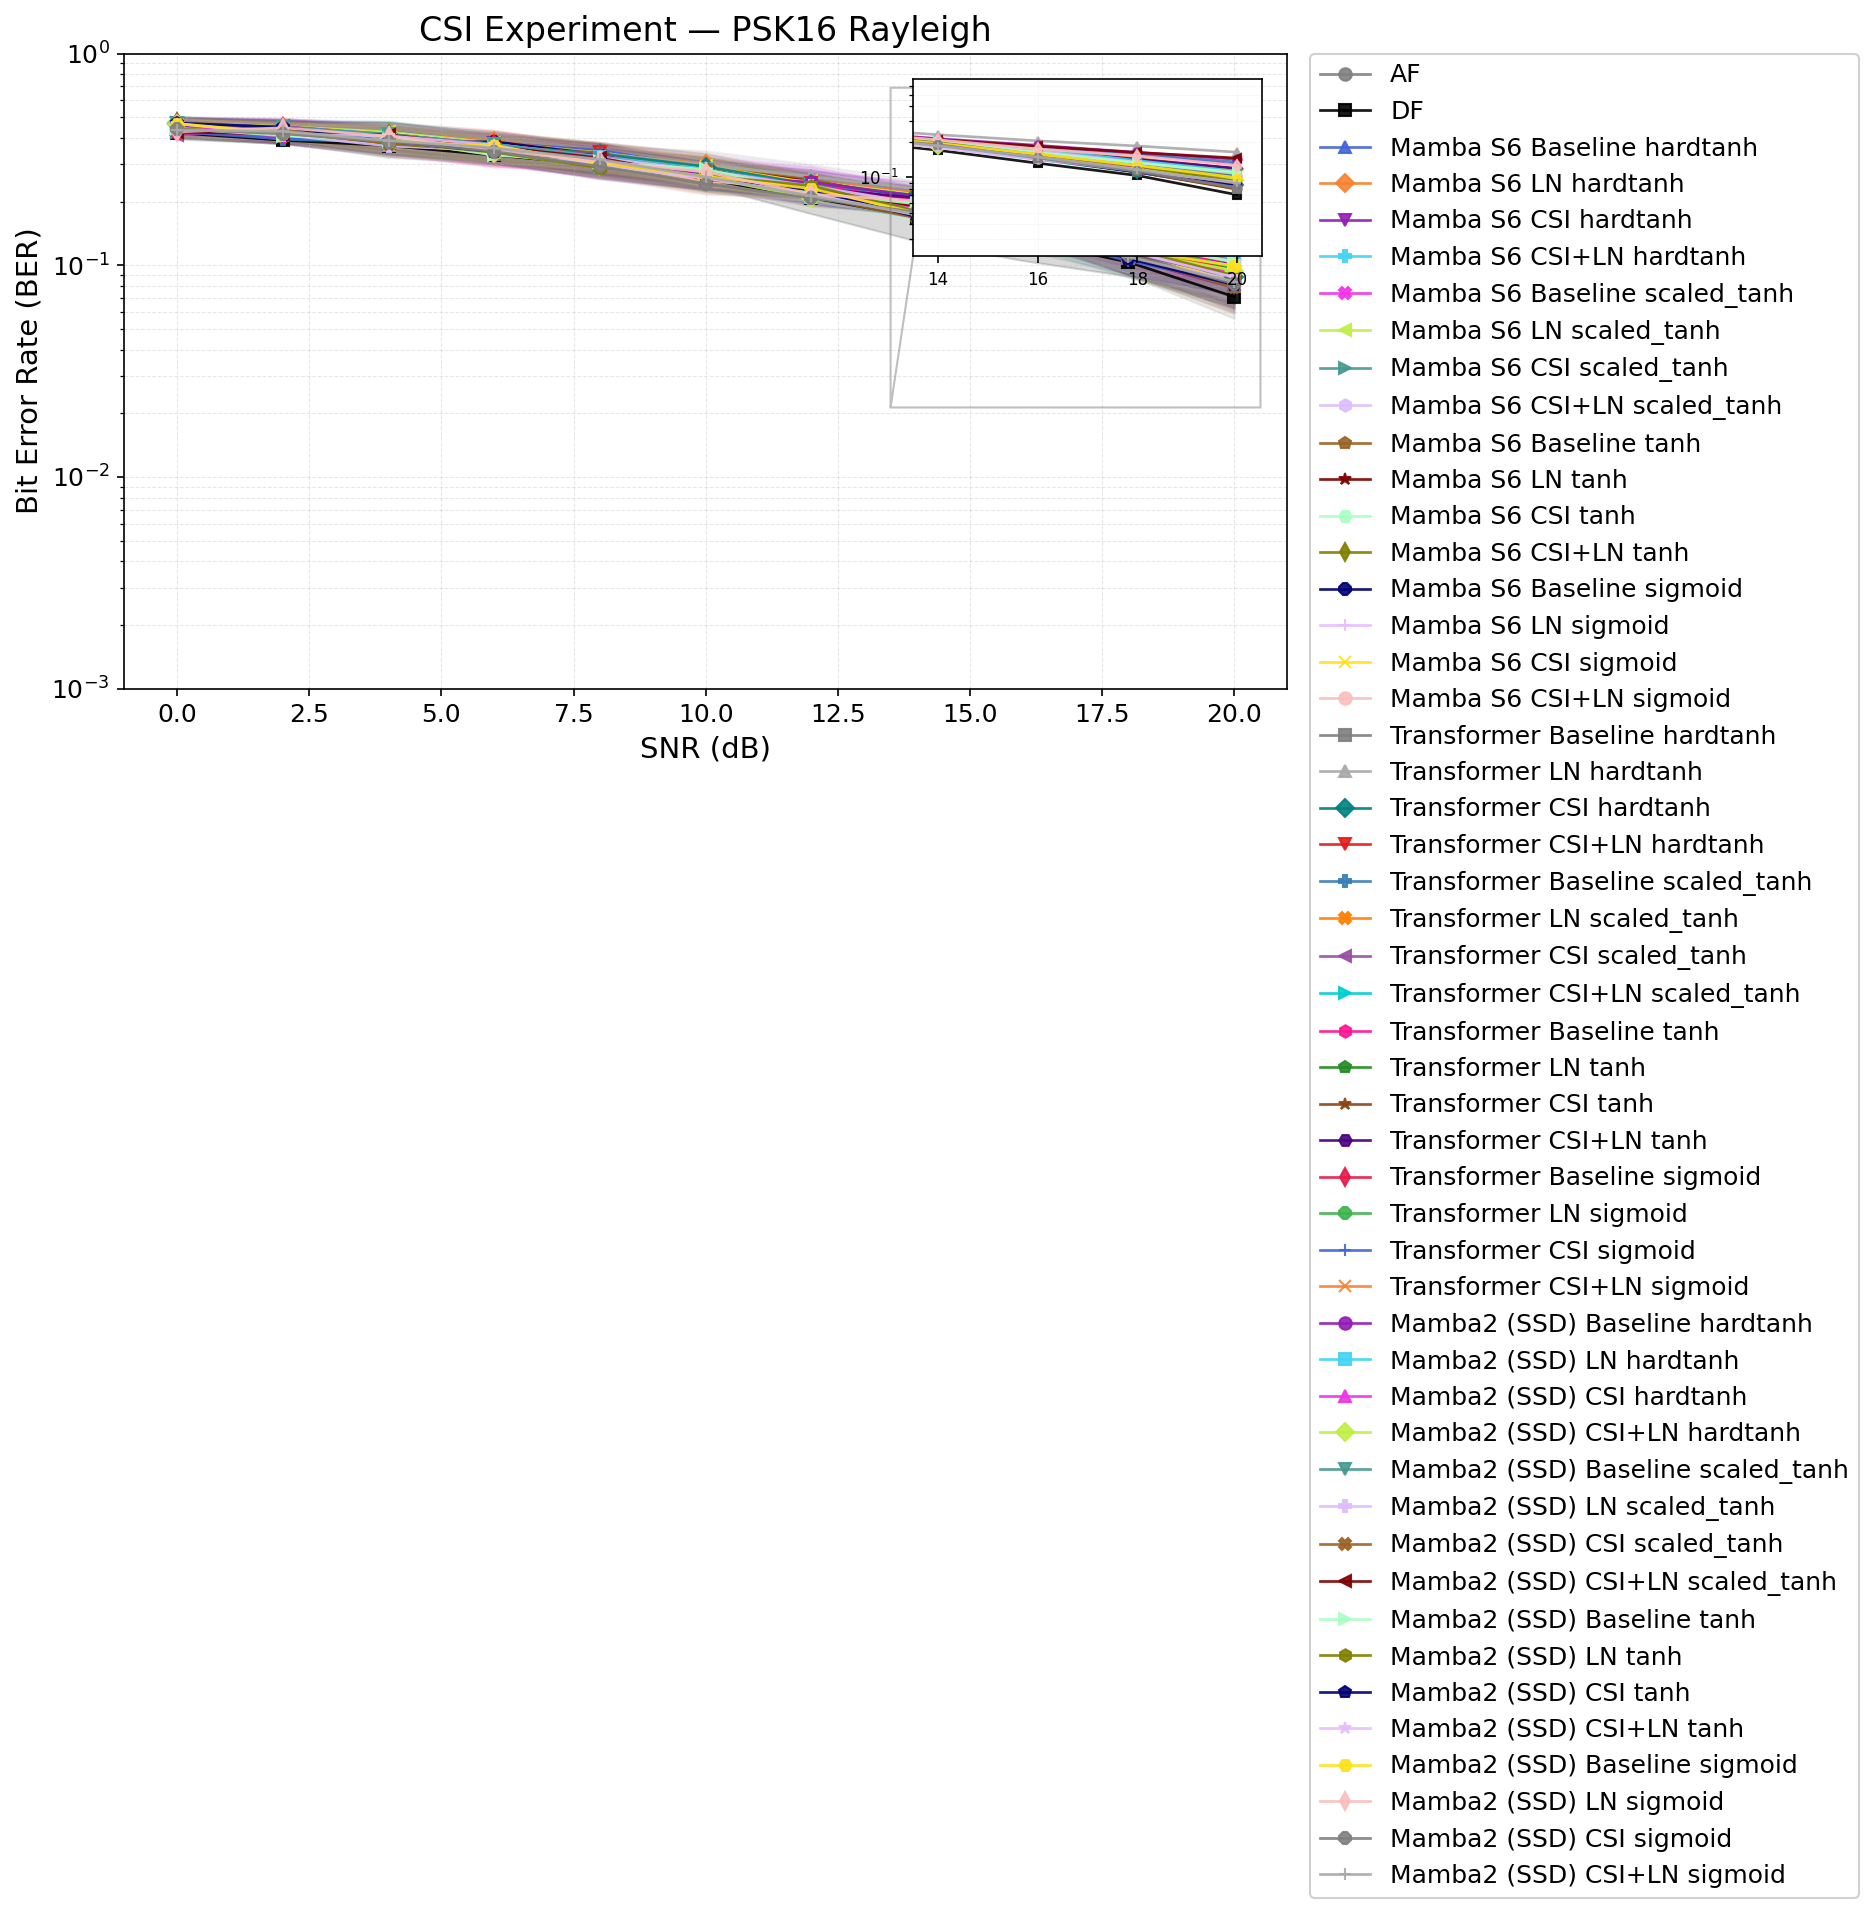
\includegraphics[width=\linewidth,height=0.45\textheight,keepaspectratio]{results/csi/csi_experiment_psk16_rayleigh.png}}
\caption{16-PSK Rayleigh fading --- BER vs.~SNR for all 48 neural relay variants and two classical baselines. The neural variants form a tighter cluster than QAM16, reflecting the constant-envelope nature of PSK which reduces the amplitude-aliasing challenge.}\label{fig:fig41}
\end{figure}

\begin{figure}[H]
\centering
\centering
\pandocbounded{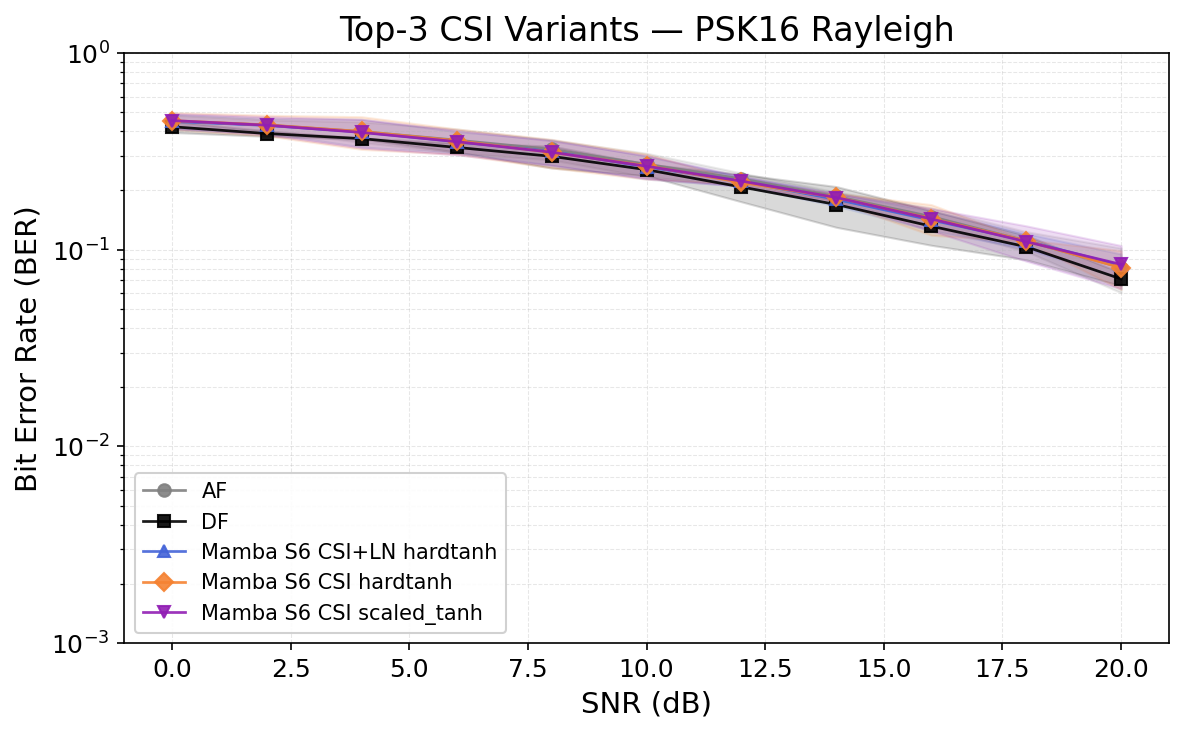
\includegraphics[width=\linewidth,height=0.45\textheight,keepaspectratio]{results/csi/top3_psk16_rayleigh.png}}
\caption{Top-3 neural relay architectures compared against AF and DF for 16-PSK in Rayleigh fading. In contrast to QAM16, all three best-performing PSK16 variants use CSI injection (+CSI or +CSI+LN).}\label{fig:fig42}
\end{figure}

\begin{figure}[H]
\centering
\centering
\pandocbounded{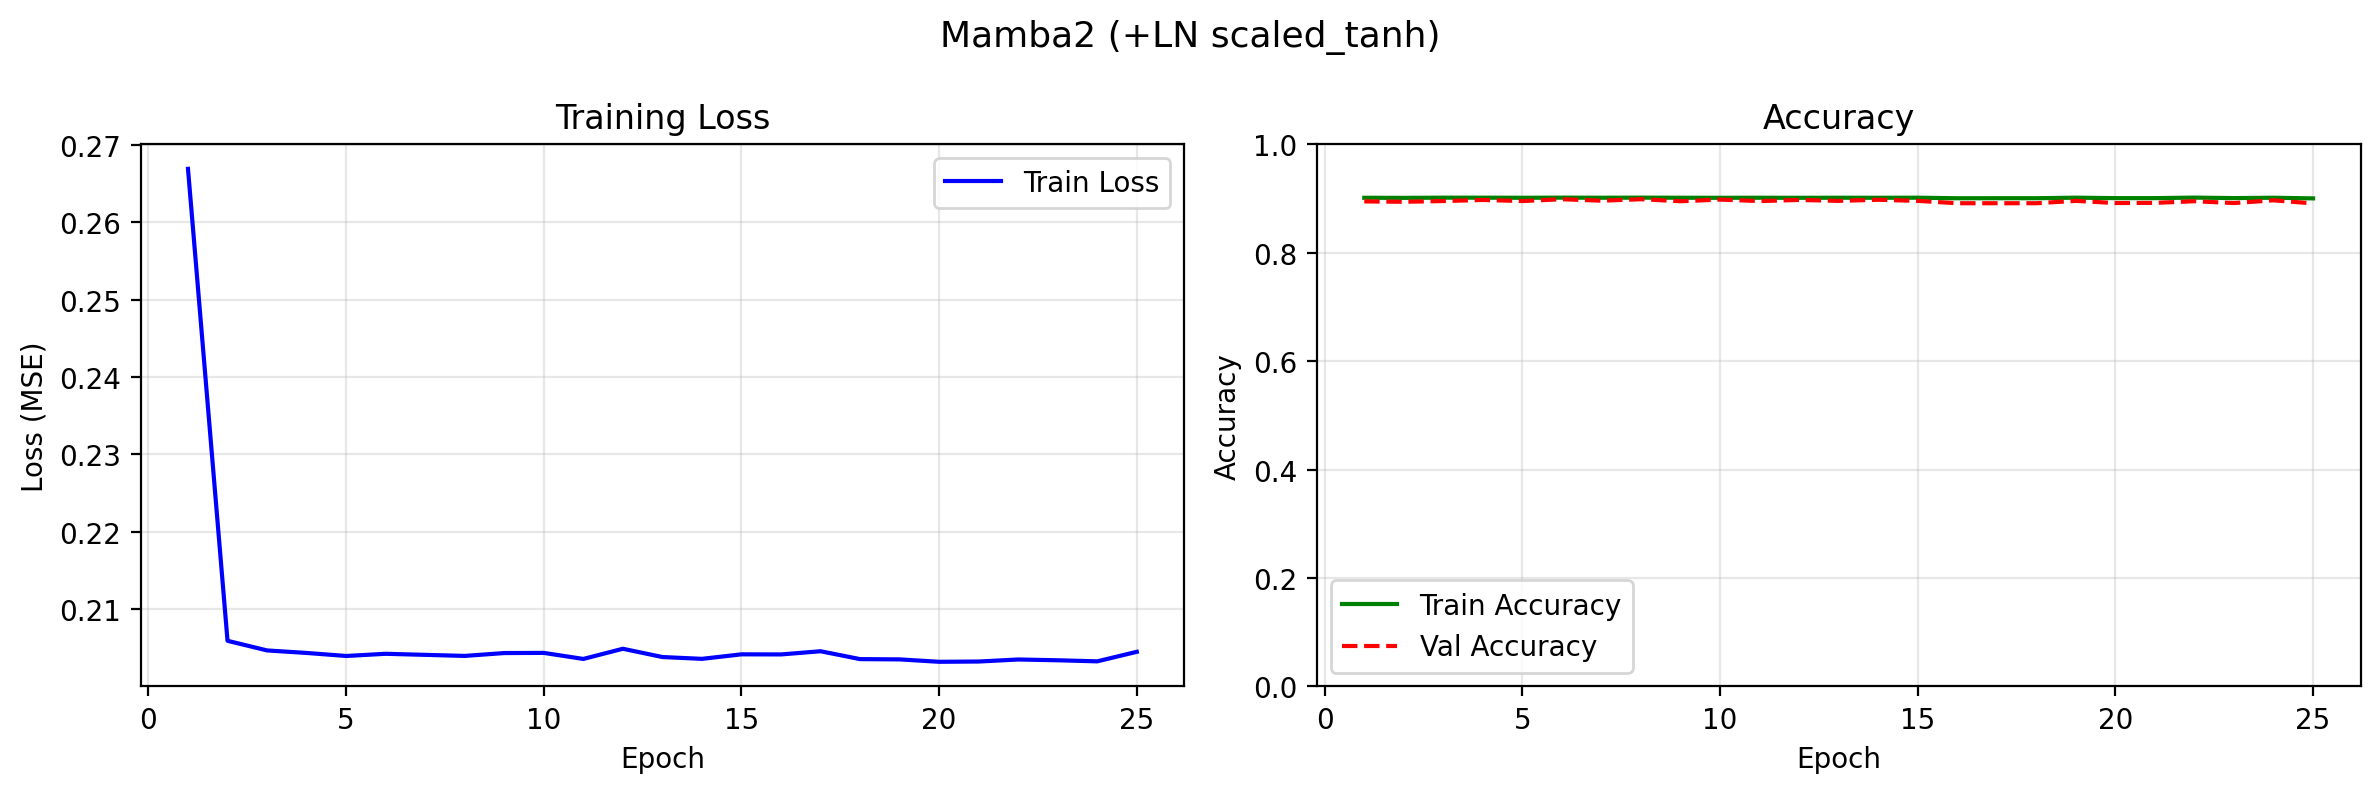
\includegraphics[width=\linewidth,height=0.45\textheight,keepaspectratio]{results/csi/training_Mamba2_LN_scaled_tanh.png}}
\caption{Training loss (MSE) and accuracy for Mamba-2 (+LN scaled\_tanh). The model converges within approximately 5 epochs and stabilises, with validation accuracy closely tracking training accuracy --- indicating minimal overfitting.}\label{fig:fig43}
\end{figure}

\begin{figure}[H]
\centering
\centering
\pandocbounded{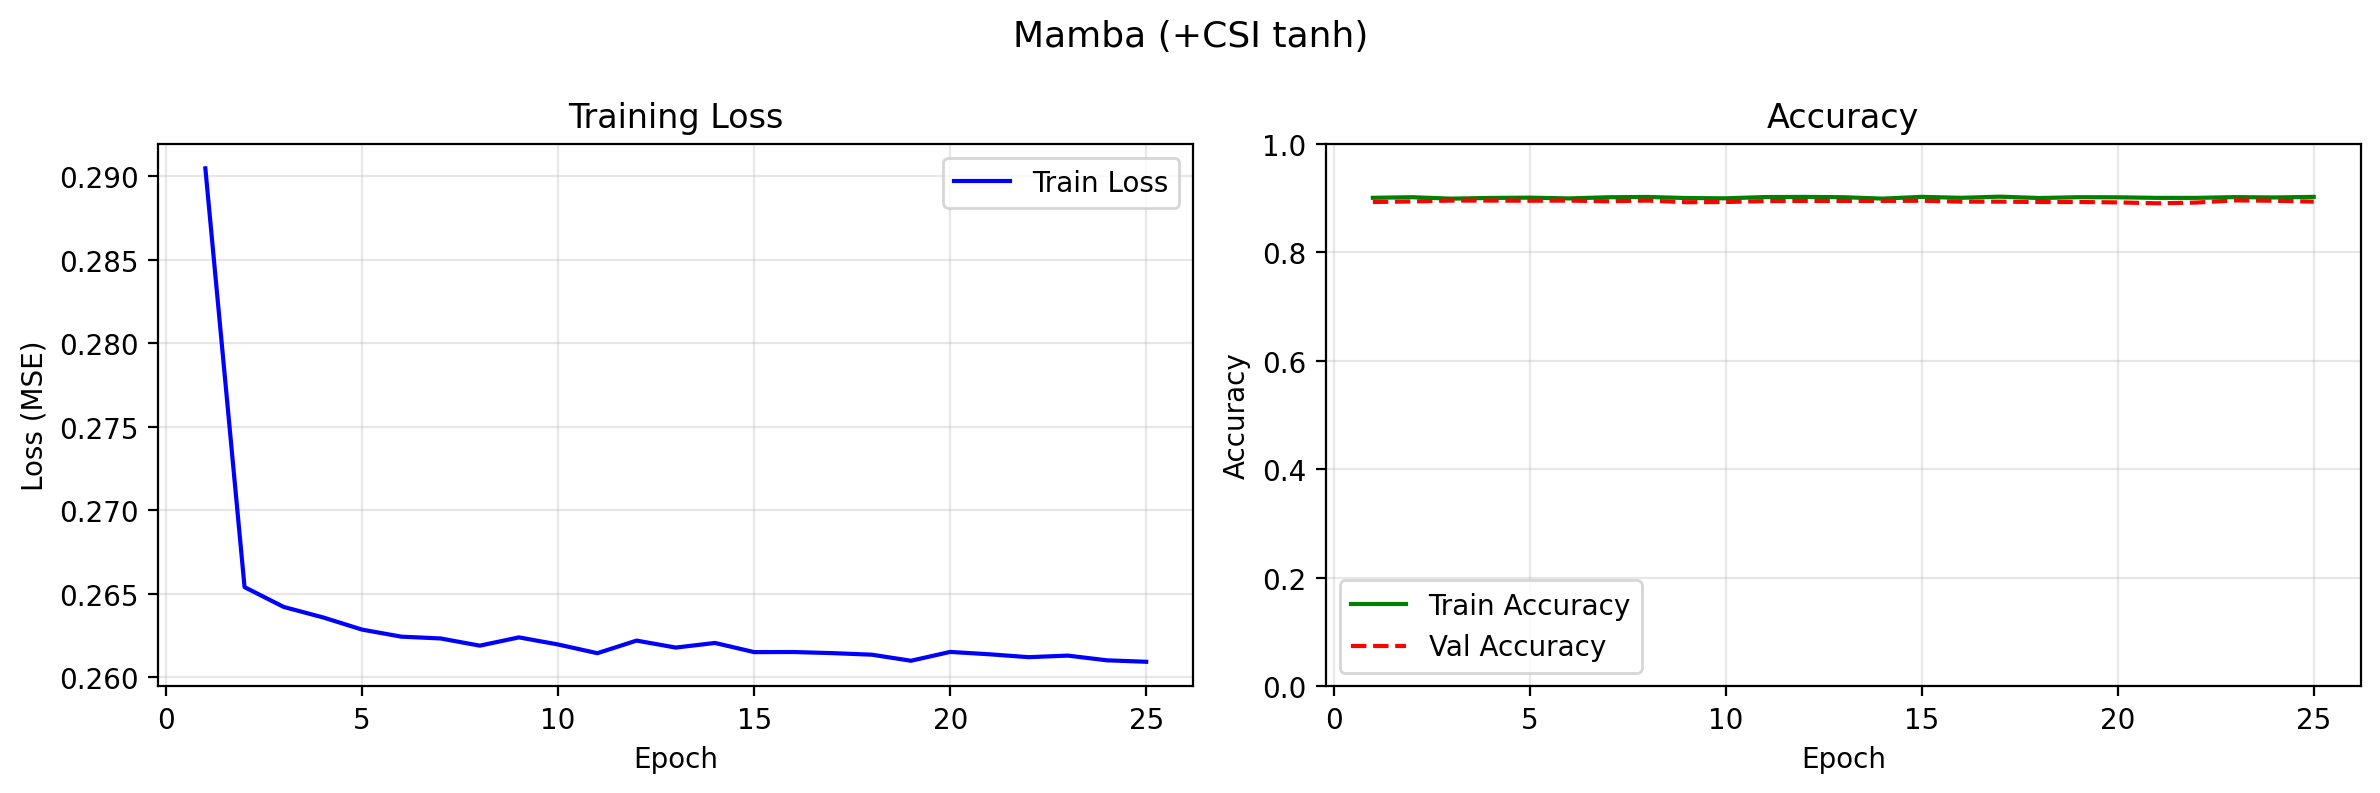
\includegraphics[width=\linewidth,height=0.45\textheight,keepaspectratio]{results/csi/training_Mamba_CSI_tanh.png}}
\caption{Training loss and accuracy for Mamba S6 (+CSI tanh). The CSI-augmented input produces a smooth, monotonic training convergence, with the additional channel-state feature providing clear gradient signal for the optimizer.}\label{fig:fig44}
\end{figure}

\begin{figure}[H]
\centering
\centering
\pandocbounded{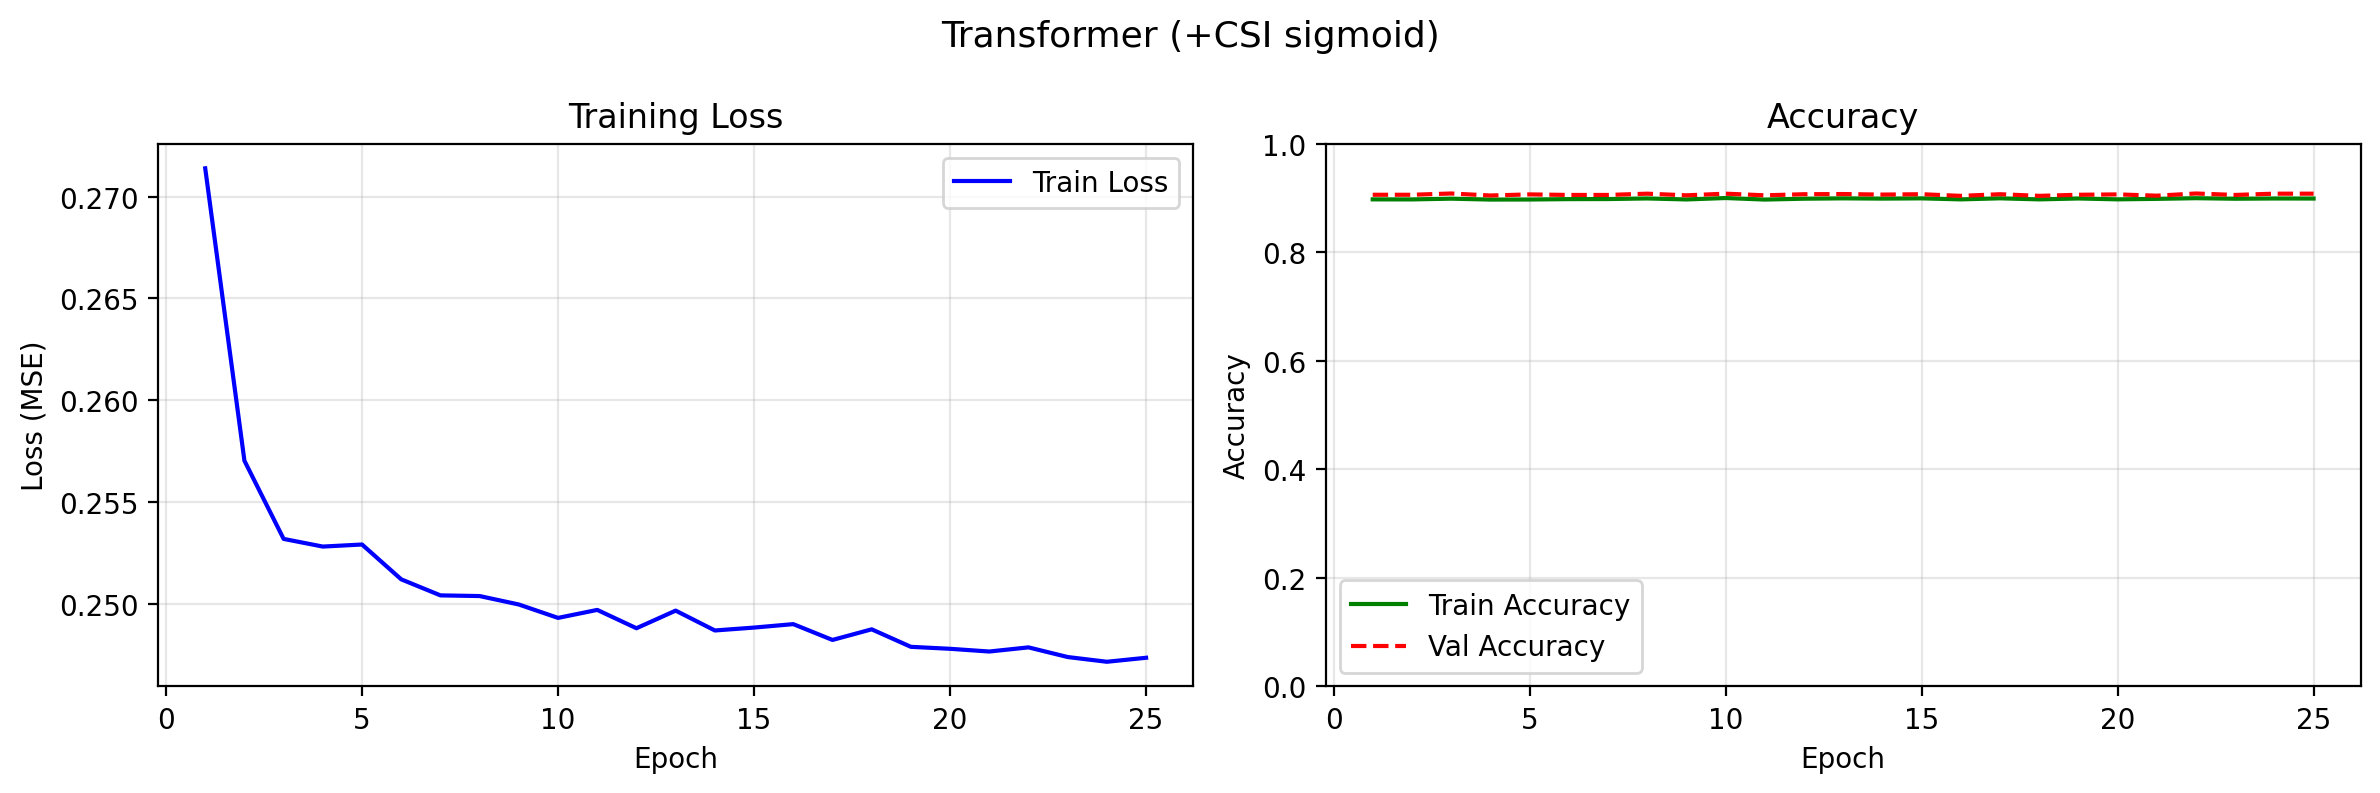
\includegraphics[width=\linewidth,height=0.45\textheight,keepaspectratio]{results/csi/training_Transformer_CSI_sigmoid.png}}
\caption{Training loss and accuracy for Transformer (+CSI sigmoid). The Transformer exhibits rapid initial convergence (within 3 epochs) followed by a flat plateau, characteristic of the attention mechanism's ability to capture input structure quickly.}\label{fig:fig45}
\end{figure}

\section{16-Class 2D Classification for QAM16}\label{sec:class-2d-classification-for-qam16}

\textbf{Goal:} Eliminate the structural BER floor imposed by per-axis I/Q splitting for 16-QAM by utilizing full 2D decision boundaries.

\textbf{Trials:} - \textbf{Topology:} SISO - \textbf{Modulation scheme:} 16-QAM - \textbf{Channel:} AWGN - \textbf{Equalizers:} None - \textbf{NN architecture:} Supervised (MLP), Generative (VAE), Sequence (Transformer, Mamba S6, Mamba-2 SSD) - \textbf{NN activation:} None (Softmax implicitly via Cross-Entropy loss) - \textbf{Special case:} 16-class joint 2D classification

\textbf{Conclusion:} Treating the relay as a joint 16-point classifier over the full 2D constellation space completely eliminates the structural 4-class BER floor. For the first time, neural variants (VAE, Transformer, MLP) matched classical DF performance at high SNR, achieving near-zero BER at 20 dB. This proves the previous BER floor was an artifact of I/Q splitting, not a fundamental limitation (Equation~\ref{eq:iq-splitting}) of neural relays.

\subsection{Results Tables}\label{sec:results-tables-5}

Table 24 presents the BER at 20 dB for all variants alongside the classical AF and DF baselines.

\begin{longtable}[]{@{}llll@{}}
\caption{BER at 20 dB for all relay variants: 4-class (I/Q split) vs.~16-class (joint 2D) classification for 16-QAM.}\label{tbl:table24}\tabularnewline
\toprule\noalign{}
Relay & 4-cls BER @ 20 dB & 16-cls BER @ 20 dB & Improvement \\
\midrule\noalign{}
\endfirsthead
\toprule\noalign{}
Relay & 4-cls BER @ 20 dB & 16-cls BER @ 20 dB & Improvement \\
\midrule\noalign{}
\endhead
\bottomrule\noalign{}
\endlastfoot
MLP & 0.00811 & \textbf{0.00002} & 405× \\
VAE & --- & \textbf{0.00000} & --- \\
CGAN & 0.00811 & --- & --- \\
Hybrid & --- & --- & --- \\
Transformer & 0.00810 & \textbf{0.00001} & 810× \\
Mamba S6 & 0.00810 & \textbf{0.00009} & 90× \\
Mamba-2 SSD & 0.00811 & \textbf{0.00197} & 4.1× \\
AF & 0.00063 & --- & --- \\
DF & 0.00000 & --- & --- \\
\end{longtable}

\subsection{Results Figures}\label{sec:results-figures-6}

\begin{figure}[H]
\centering
\centering
\pandocbounded{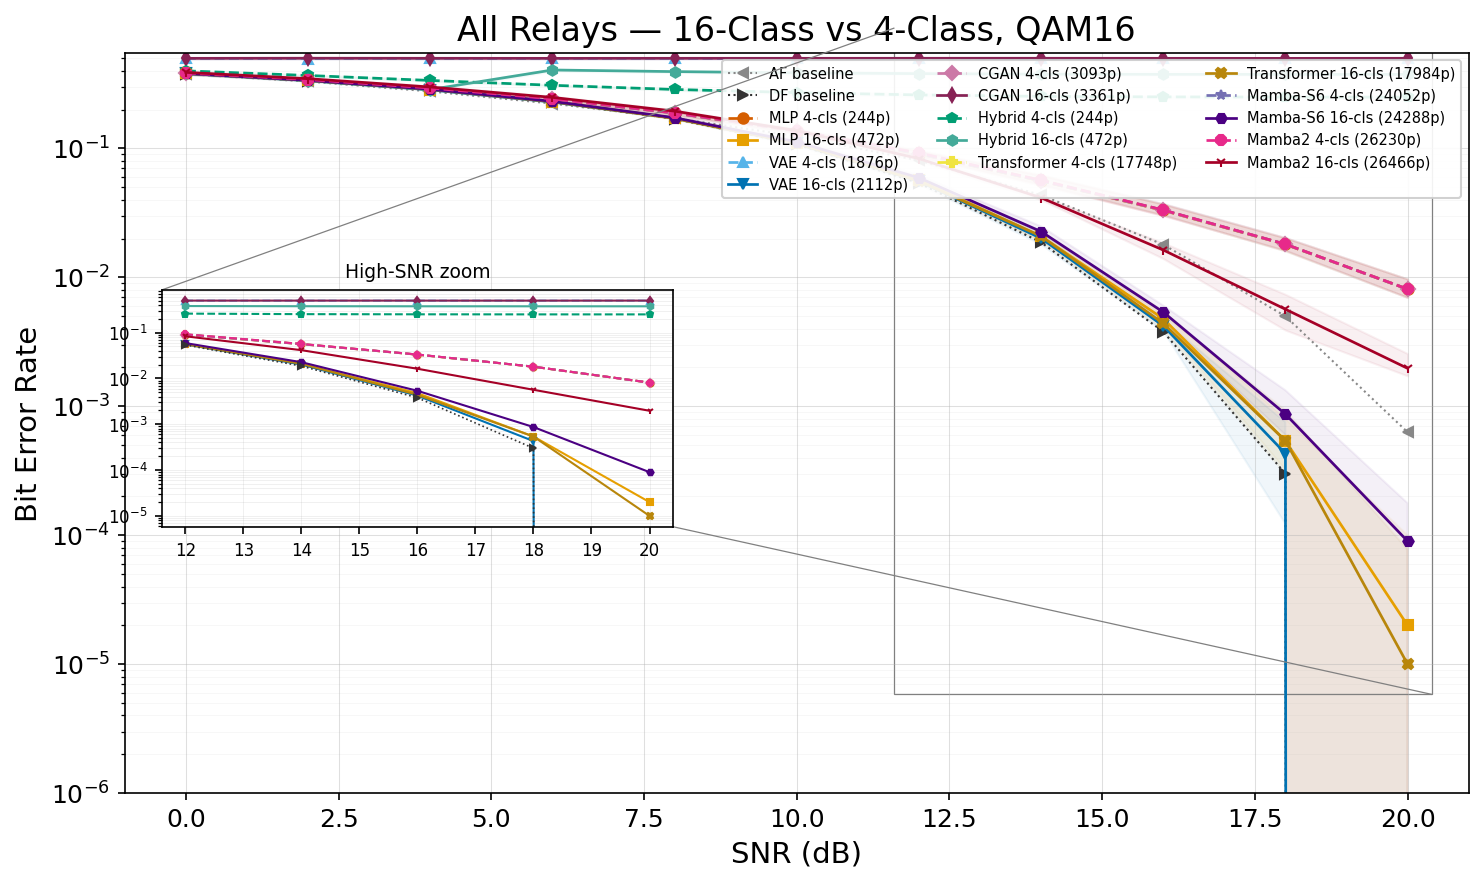
\includegraphics[width=\linewidth,height=0.45\textheight,keepaspectratio]{results/all_relays_16class/ber_all_relays_16class.png}}
\caption{16-QAM BER vs.~SNR for all relay variants (4-class and 16-class) on AWGN. The 4-class variants (dashed) plateau at BER ≈ 0.008 while the successfully trained 16-class variants (solid) continue decreasing, approaching and matching the DF baseline.}\label{fig:fig50}
\end{figure}

\begin{figure}[H]
\centering
\centering
\pandocbounded{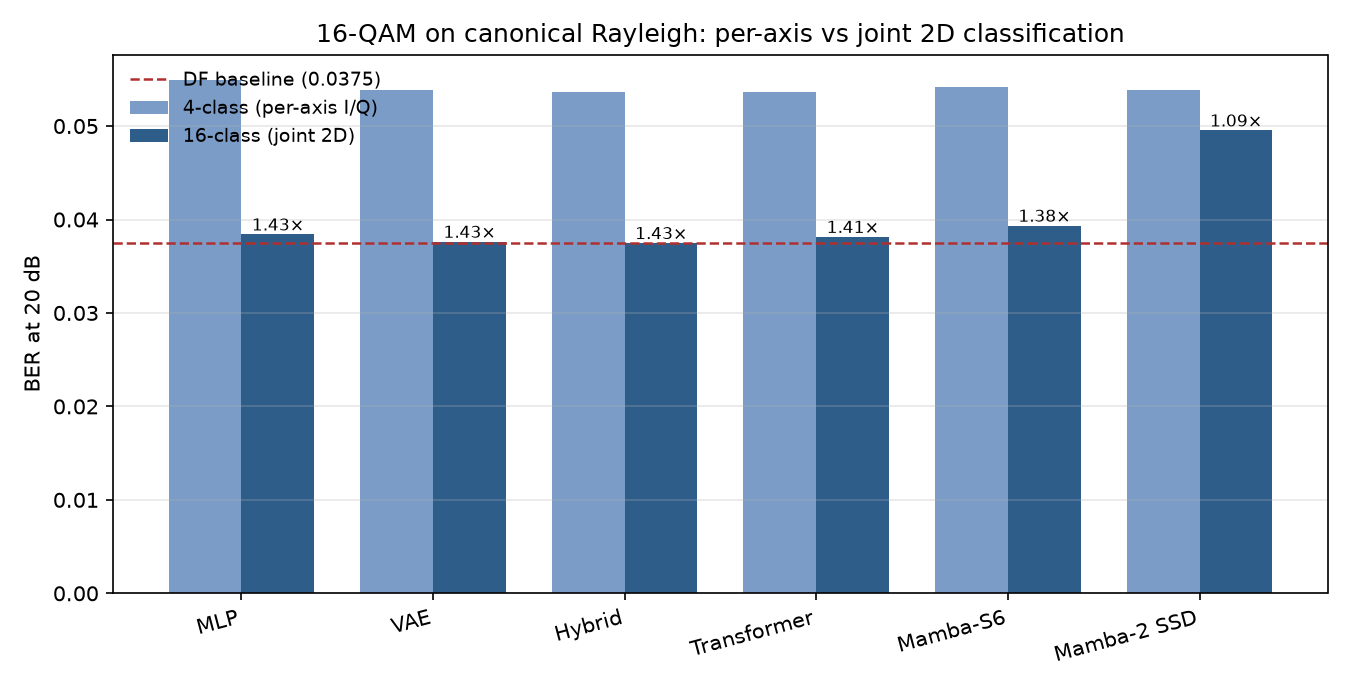
\includegraphics[width=\linewidth,height=0.45\textheight,keepaspectratio]{results/all_relays_16class/grouped_bar_16class.png}}
\caption{Grouped bar comparison of 4-class vs.~16-class BER at 20 dB for each architecture. The 16-class advantage is visible for MLP, VAE, Transformer, and Mamba S6. Failed variants (VAE 4-cls \textasciitilde0.50, CGAN 16-cls \textasciitilde0.50) are truncated.}\label{fig:fig51}
\end{figure}

\begin{figure}[H]
\centering
\centering
\pandocbounded{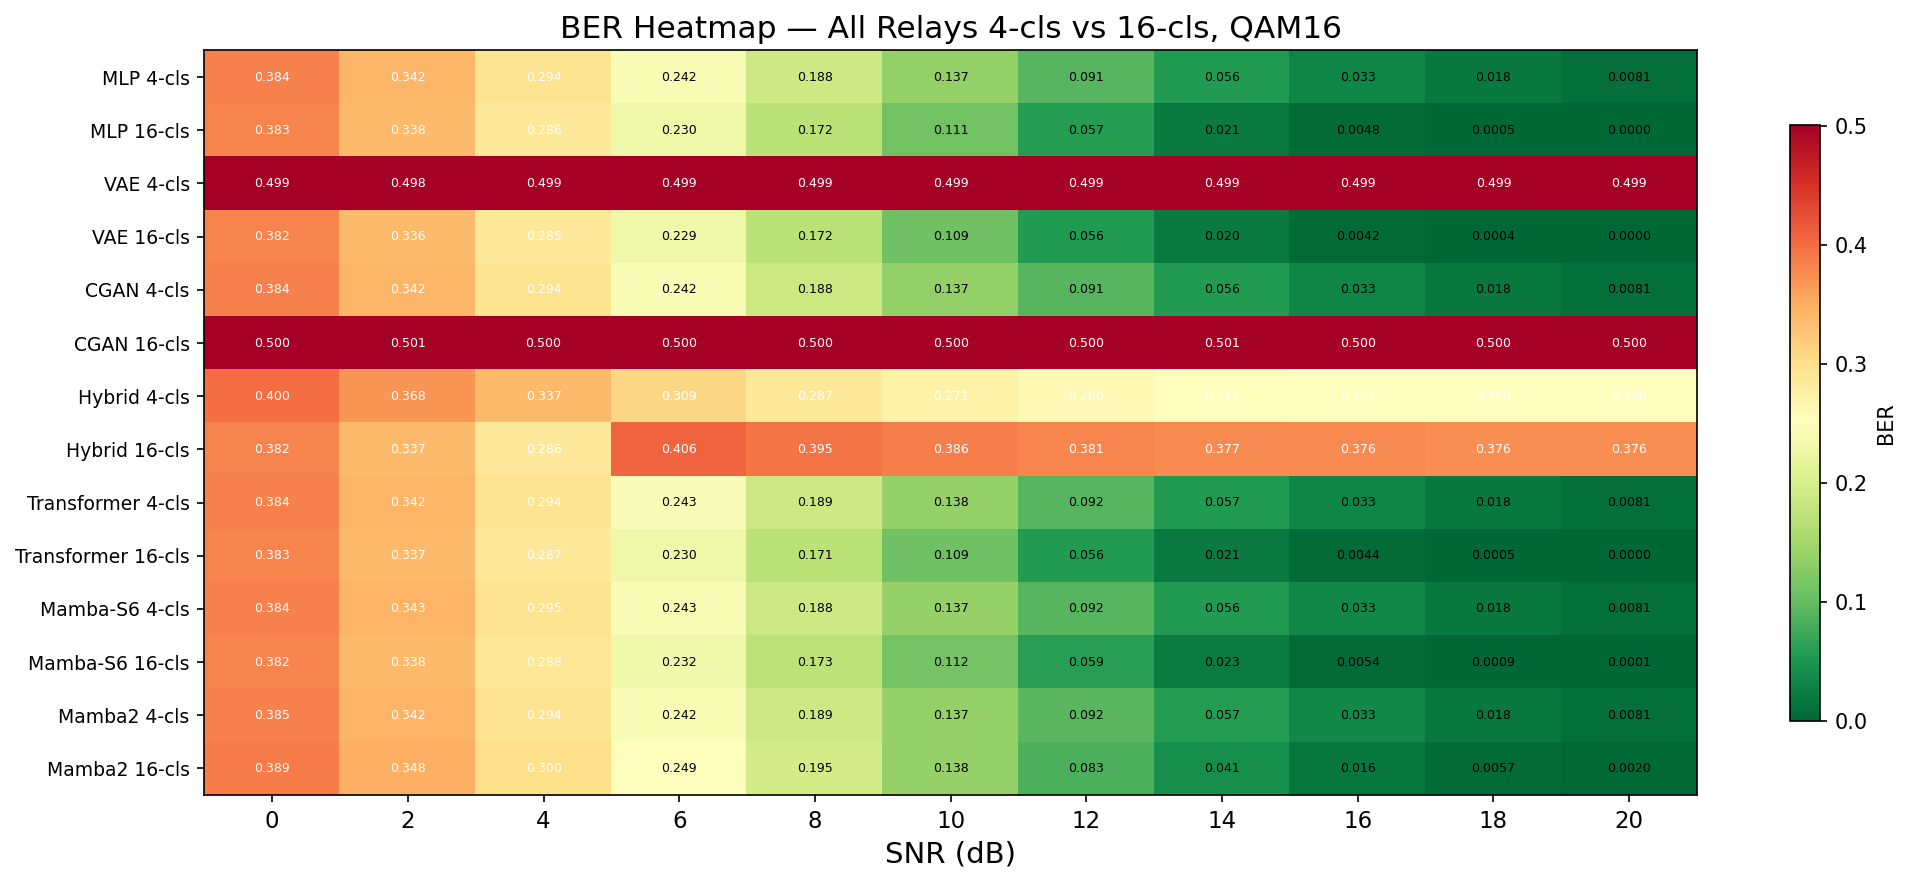
\includegraphics[width=\linewidth,height=0.45\textheight,keepaspectratio]{results/all_relays_16class/heatmap_all_relays_16class.png}}
\caption{Heatmap of BER across all relay variants and SNR points. The 16-class variants show a clear colour transition from high BER (warm) at low SNR to near-zero BER (cool) at high SNR, while 4-class variants remain warm at high SNR due to the structural floor.}\label{fig:fig52}
\end{figure}

\begin{figure}[H]
\centering
\centering
\pandocbounded{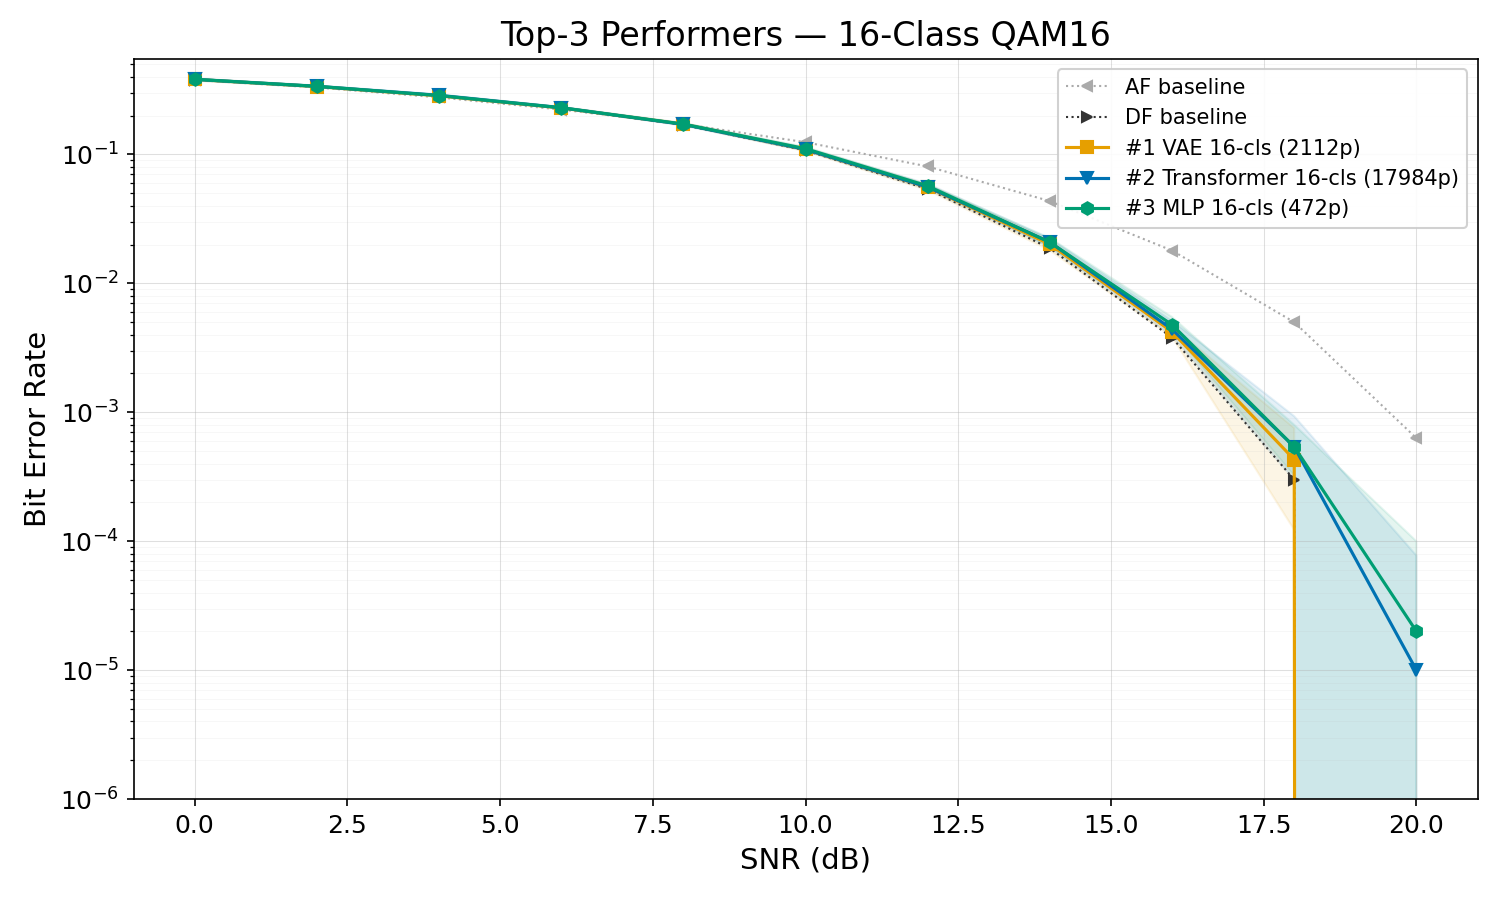
\includegraphics[width=\linewidth,height=0.45\textheight,keepaspectratio]{results/all_relays_16class/top3_16class.png}}
\caption{Top-3 16-class relay variants compared against AF and DF. VAE 16-cls, Transformer 16-cls, and MLP 16-cls all match or approach DF performance across the full SNR range.}\label{fig:fig53}
\end{figure}

\section{End-to-End Joint Optimization}\label{sec:end-to-end-joint-optimization}

\textbf{Goal:} Compare the modular neural relay approach against a fully joint transmitter-receiver autoencoder.

\textbf{Trials:} - \textbf{Topology:} SISO - \textbf{Modulation scheme:} Learned latent space (M=16, power-constrained) - \textbf{Channel:} Rayleigh - \textbf{Equalizers:} ZF explicitly at the receiver - \textbf{NN architecture:} MLP Autoencoder (Encoder/Decoder) - \textbf{Special case:} End-to-End (E2E) optimization

\textbf{Conclusion:} The E2E autoencoder underperforms both the theoretical limits of classical 16-QAM and the modular two-hop DF relay across all SNR points (67-141\% higher BER). The network fails to discover a constellation geometry that surpasses the classical square grid under single-antenna Rayleigh fading, demonstrating that `black-box' deep learning is inefficient compared to modular designs that leverage classical signal processing algorithms for modulation and equalization.

\subsection{Results Figures}\label{sec:results-figures-7}

\begin{figure}[H]
\centering
\centering
\pandocbounded{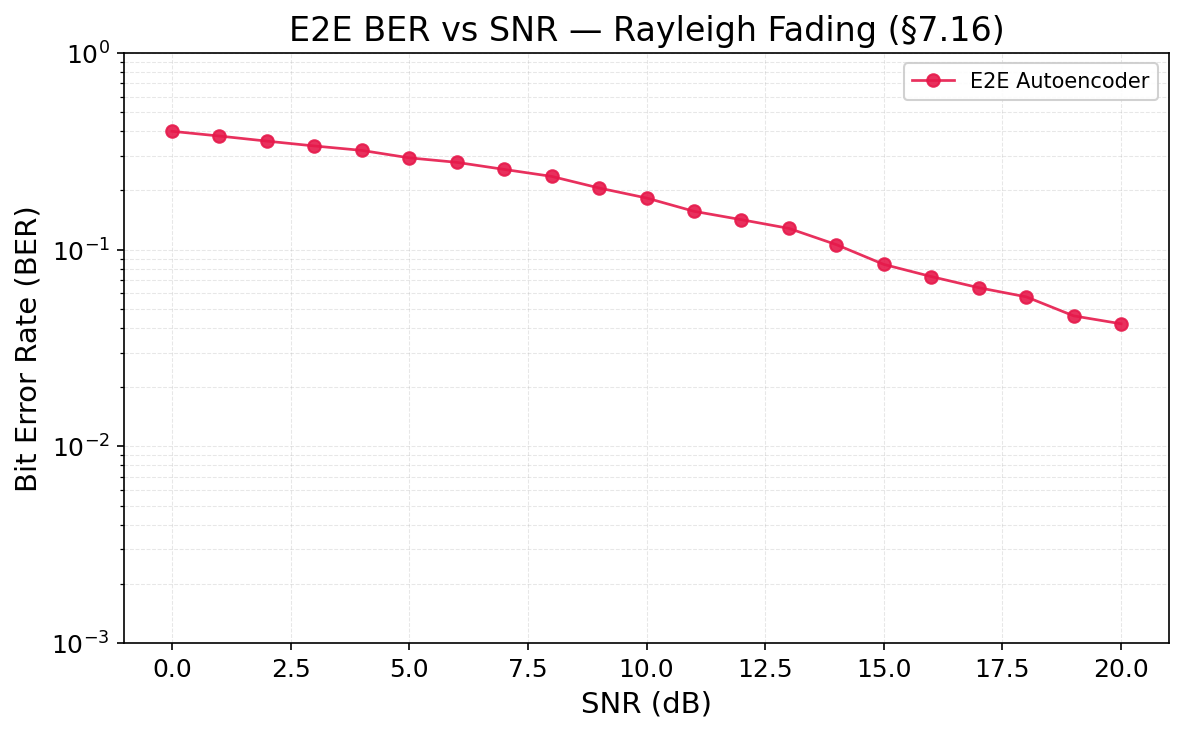
\includegraphics[width=\linewidth,height=0.45\textheight,keepaspectratio]{results/e2e/e2e_ber_comparison.png}}
\caption{BER vs.~SNR for E2E learned autoencoder compared to theoretical 16-QAM over Rayleigh fading. The E2E system underperforms the classical grid constellation across the full SNR range, with the gap widening at high SNR.}\label{fig:fig46}
\end{figure}

\begin{figure}[H]
\centering
\centering
\pandocbounded{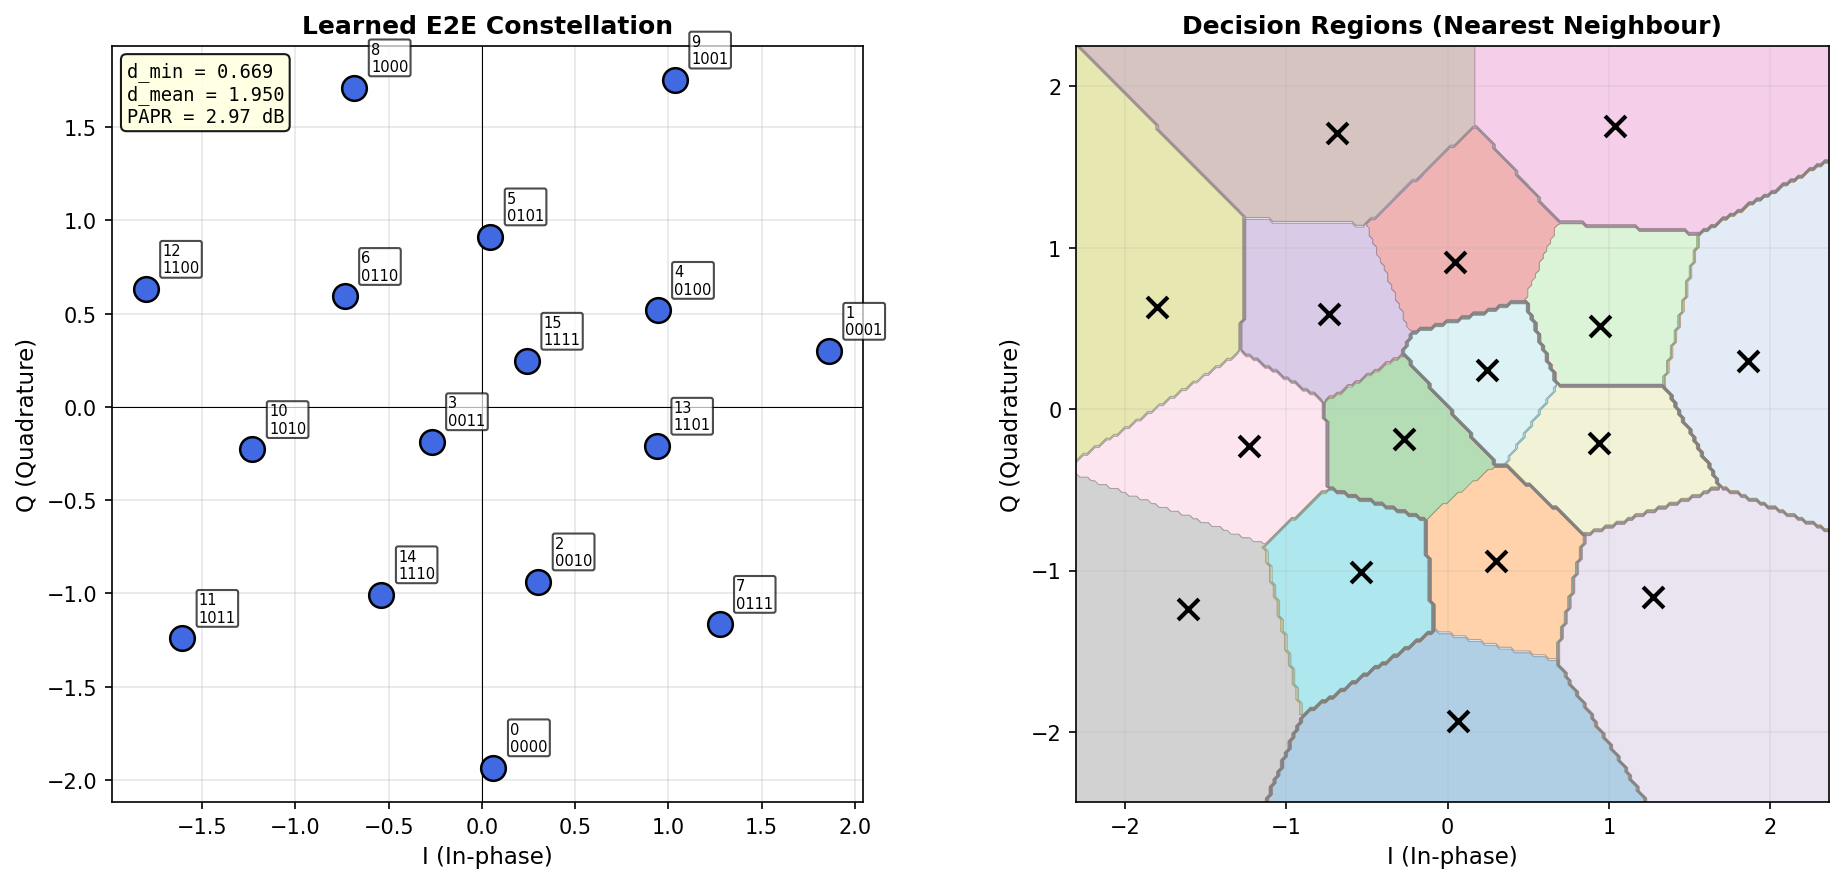
\includegraphics[width=\linewidth,height=0.45\textheight,keepaspectratio]{results/e2e/e2e_constellation.png}}
\caption{Learned 16-point constellation of the E2E autoencoder. The network discovers a non-rectangular geometry (resembling a hexagonal lattice or concentric APSK layout) that maximises minimum Euclidean distance under the average power constraint, unlike the classical \(4 \times 4\) square grid.}\label{fig:fig47}
\end{figure}

\begin{figure}[H]
\centering
\centering
\pandocbounded{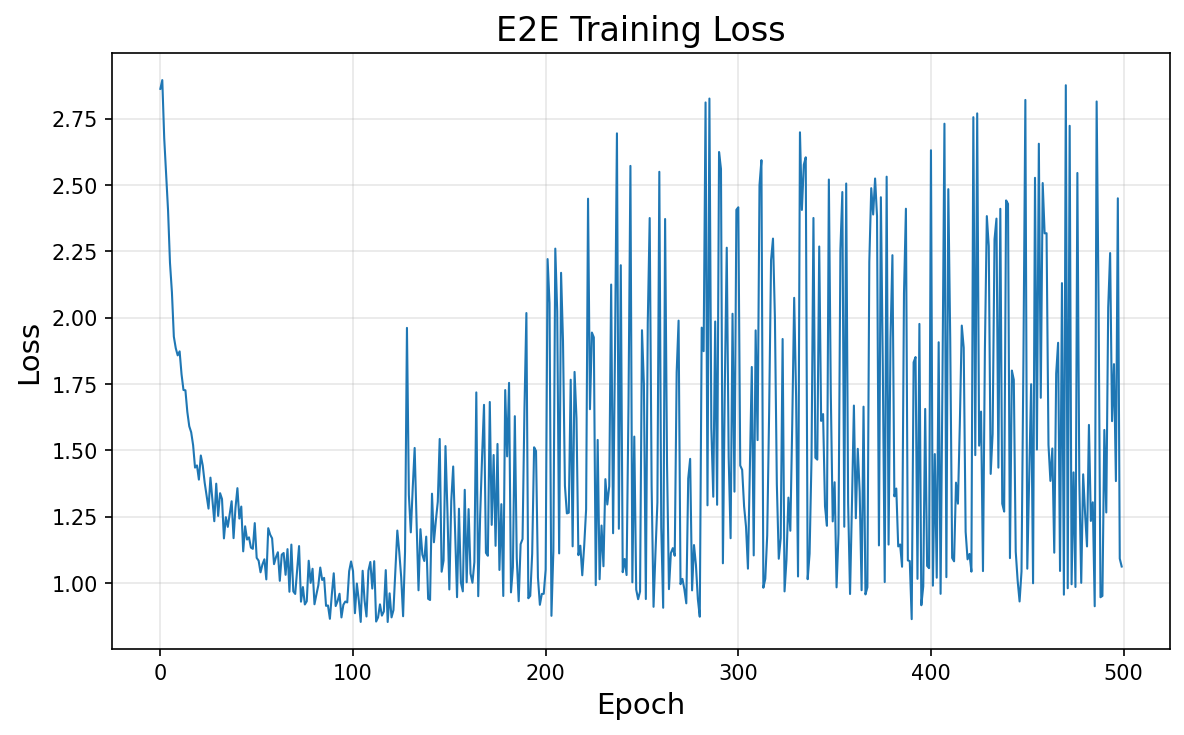
\includegraphics[width=\linewidth,height=0.45\textheight,keepaspectratio]{results/e2e/e2e_training_loss.png}}
\caption{Training loss (cross-entropy) convergence of the E2E autoencoder. The model converges within approximately 200 epochs.}\label{fig:fig48}
\end{figure}

\begin{figure}[H]
\centering
\centering
\pandocbounded{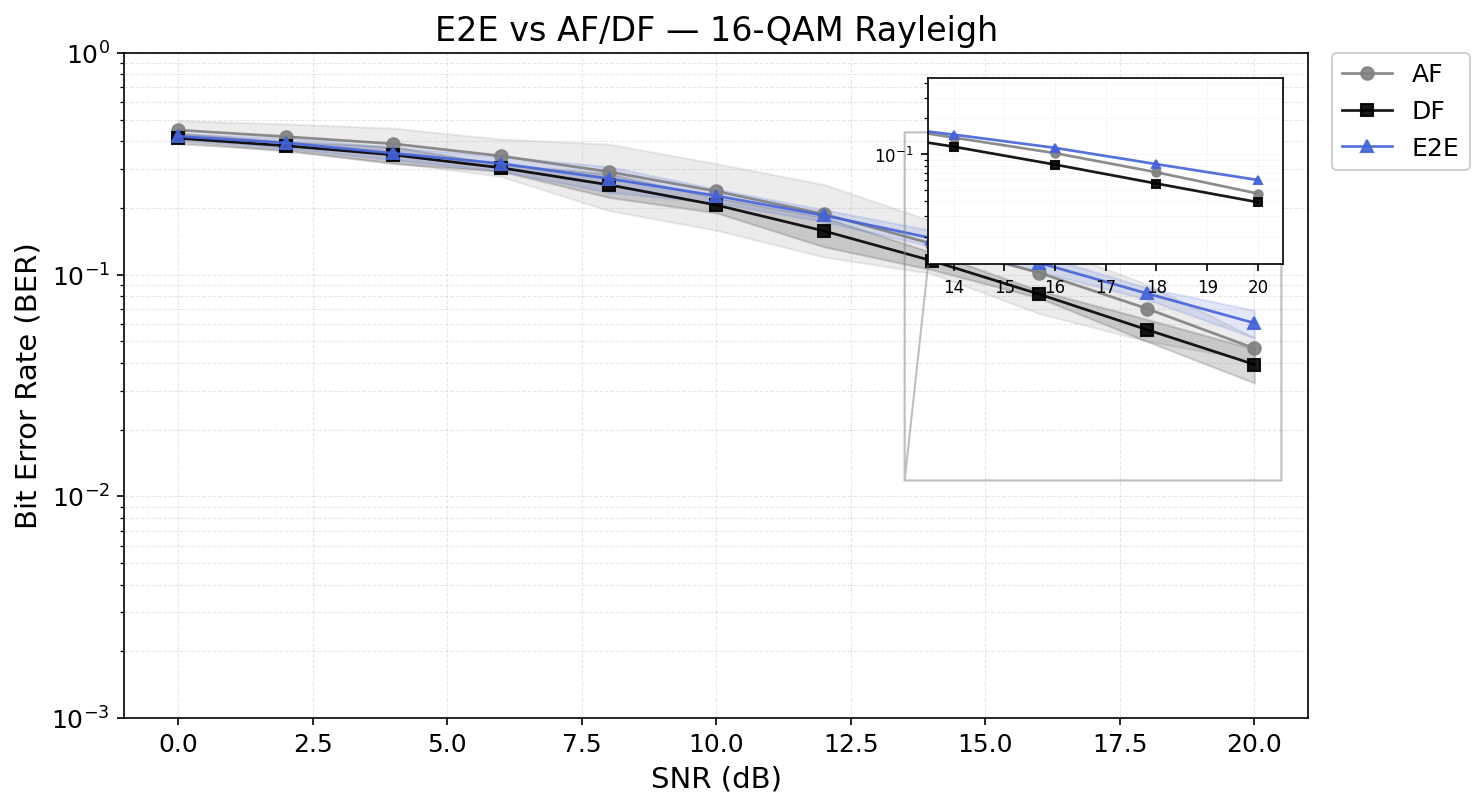
\includegraphics[width=\linewidth,height=0.45\textheight,keepaspectratio]{results/e2e/e2e_relay_comparison.png}}
\caption{Performance comparison of the E2E autoencoder against the modular relay-based approaches from this thesis. The E2E system does not achieve lower BER than the two-hop DF relay, highlighting the limitations of the E2E approach.}\label{fig:fig49}
\end{figure}

